\documentclass[final,5p]{elsarticle}

% \documentclass[preprint,12pt]{elsarticle}

%% Use the option review to obtain double line spacing
%% \documentclass[authoryear,preprint,review,12pt]{elsarticle}

%% Use the options 1p,twocolumn; 3p; 3p,twocolumn; 5p; or 5p,twocolumn
%% for a journal layout:
% \documentclass[final,1p,times]{elsarticle}
%% \documentclass[final,1p,times,twocolumn]{elsarticle}
% \documentclass[final,3p,times]{elsarticle}
%% \documentclass[final,3p,times,twocolumn]{elsarticle}
% \documentclass[final,5p,times]{elsarticle}
%% \documentclass[final,5p,times,twocolumn]{elsarticle}
\usepackage[portuguese]{babel}

%% For including figures, graphicx.sty has been loaded in
%% elsarticle.cls. If you prefer to use the old commands
%% please give \usepackage{epsfig}

%% The amssymb package provides various useful mathematical symbols
\usepackage{amssymb}
\usepackage{amsmath}
\usepackage{multirow}
\usepackage{tabularx}
\usepackage{booktabs}
\usepackage{tablefootnote}

\usepackage{pgfplots}
\pgfplotsset{compat=1.18}
\usepgfplotslibrary{statistics}
\usepackage{pgfplotstable}

\usepackage{placeins}
\usepackage{hyperref}
\numberwithin{equation}{section}

\usepackage{algorithm}
\usepackage[noEnd=true, indLines=true]{algpseudocodex}
\algrenewcommand\algorithmicrequire{\textbf{Entrada:}}
\algrenewcommand\algorithmicwhile{\textbf{Enquanto}}
\algrenewcommand\algorithmicrepeat{\textbf{Repete}}
\algrenewcommand\algorithmicuntil{\textbf{Até}}
\algrenewcommand\algorithmicif{\textbf{Se}}
\algrenewcommand\algorithmicthen{\textbf{então}}
\algrenewcommand\algorithmicelse{\textbf{Caso contrário}}
\algrenewcommand\algorithmicensure{\textbf{Objetivo:}}
\algrenewcommand\algorithmicreturn{\textbf{Retorna:}}
\algrenewcommand\algorithmicdo{\textbf{faça}}
\algrenewcommand\algorithmicforall{\textbf{Para todos}}
\algnewcommand{\LineComment}[1]{\State \(\triangleright\) \textcolor{black!50}{\emph{#1}}}

\newcommand*{\squareb}{\textcolor{black}{\rule{0.5em}{0.5em}}}
\newcommand*{\squareg}{\textcolor{gray}{\rule{0.5em}{0.5em}}}

\graphicspath{ {./png/} }

% \usepackage[fleqn]{nccmath}
% \usepackage{multicol}


%=========== Gloabal Tikz settings
% \pgfplotsset{compat=newest}
% \usetikzlibrary{math}
% \pgfplotsset{
%     height = 10cm,
%     width = 10cm,
%     tick pos = left,
%     legend style={at={(0.98,0.30)}, anchor=east},
%     legend cell align=left,
%     }
%  \pgfkeys{
%     /pgf/number format/.cd,
%     fixed,
%     precision = 1,
%     set thousands separator = {}
% }

%% The amsthm package provides extended theorem environments
%% \usepackage{amsthm}

%% The lineno packages adds line numbers. Start line numbering with
%% \begin{linenumbers}, end it with \end{linenumbers}. Or switch it on
%% for the whole article with \linenumbers.
%% \usepackage{lineno}

\usepackage{listings}
\usepackage{xcolor}

\definecolor{codegreen}{rgb}{0,0.6,0}
\definecolor{codegray}{rgb}{0.5,0.5,0.5}
\definecolor{codepurple}{rgb}{0.58,0,0.82}
\definecolor{backcolour}{rgb}{0.98,0.98,0.98}

\lstdefinestyle{mystyle}{
    backgroundcolor=\color{backcolour},
    commentstyle=\color{codegreen},
    keywordstyle=\color{magenta},
    numberstyle=\tiny\color{codegray},
    stringstyle=\color{codepurple},
    basicstyle=\ttfamily\footnotesize,
    breakatwhitespace=false,
    breaklines=true,
    captionpos=b,
    keepspaces=true,
    numbers=left,
    numbersep=5pt,
    showspaces=false,
    showstringspaces=false,
    showtabs=false,
    tabsize=2
}

\lstset{style=mystyle}

% \journal{Nuclear Physics B}

\begin{document}

\begin{frontmatter}

%% Title, authors and addresses

%% use the tnoteref command within \title for footnotes;
%% use the tnotetext command for theassociated footnote;
%% use the fnref command within \author or \address for footnotes;
%% use the fntext command for theassociated footnote;
%% use the corref command within \author for corresponding author footnotes;
%% use the cortext command for theassociated footnote;
%% use the ead command for the email address,
%% and the form \ead[url] for the home page:
%% \title{Title\tnoteref{label1}}
%% \tnotetext[label1]{}
%% \author{Name\corref{cor1}\fnref{label2}}
%% \ead{email address}
%% \ead[url]{home page}
%% \fntext[label2]{}
%% \cortext[cor1]{}
%% \affiliation{organization={},
%%             addressline={},
%%             city={},
%%             postcode={},
%%             state={},
%%             country={}}
%% \fntext[label3]{}

\title{Classificação de Imagens com Redes Neurais Artificiais\tnoteref{label_title}}
\tnotetext[label_title]{Relatório número 03 como parte dos requisitos da disciplina IA048: Aprendizado de Máquina.}

%% use optional labels to link authors explicitly to addresses:
%% \author[label1,label2]{}
%% \affiliation[label1]{organization={},
%%             addressline={},
%%             city={},
%%             postcode={},
%%             state={},
%%             country={}}
%%
%% \affiliation[label2]{organization={},
%%             addressline={},
%%             city={},
%%             postcode={},
%%             state={},
%%             country={}}

\author[label1]{Tiago C A Amorim (RA: 100675)}
\affiliation[label1]{organization={Doutorando no Departamento de Engenharia de Petróleo da Faculdade de Engenharia Mecânica, UNICAMP},
            city={Campinas},
            state={SP},
            country={Brasil}}

\author[label2]{Taylon L C Martins (RA: 177379)}
\affiliation[label2]{organization={Aluno especial, UNICAMP},
            city={Campinas},
            state={SP},
            country={Brasil}}


% \begin{abstract}

%     xxxxxxx

% \end{abstract}


%%Graphical abstract
% \begin{graphicalabstract}
%\includegraphics{grabs}
% \end{graphicalabstract}

%%Research highlights
% \begin{highlights}
% \item Research highlight 1
% \item Research highlight 2
% \end{highlights}

\begin{keyword}
    Classificação \sep Redes Neurais Artificiais \sep Rede Neurais Convolucionais \sep ResNet
%% keywords here, in the form: keyword \sep keyword

%% PACS codes here, in the form: \PACS code \sep code

%% MSC codes here, in the form: \MSC code \sep code
%% or \MSC[2008] code \sep code (2000 is the default)

\end{keyword}

\end{frontmatter}

%% main text
\section{Introdução}

    Este relatório apresenta as principais atividades realizadas no desenvolvimento das atividades propostas na Lista 03 da disciplina IA048: Aprendizado de Máquina, primeiro semestre de 2024. O foco deste exercício é de construir e avaliar o desempenho de redes neurais artificiais -- MLP (densa de uma camada intermediária) e CNN (convolucionais \emph{rasa} e \emph{profunda}) -- na classificação de imagens de células sanguíneas periféricas.

\section{Tarefa Proposta}

    Nesta atividade, vamos abordar o problema de reconhecimento de células sanguíneas periféricas utilizando a base de dados BloodMNIST \cite{medmnistv1,medmnistv2, acevedo2020dataset} (\href{https://medmnist.com/}{https://medmnist .com/}), a qual possui 17.092 imagens microscópicas coloridas (3 canais de cor). O mapeamento entre os identificadores das classes e os rótulos está indicado na Tabela \ref{tab:rotulos}.

    \begin{table}[h]
        \centering
        \begin{tabular}{l l c}
            \toprule
            \textbf{Id} & \textbf{Rótulo} \\
            \midrule
            0 & Basófilos \\
            1 & Eosinófilos \\
            2 & Eritroblastos \\
            3 & Granulócitos imaturos \\
            4 & Linfócitos \\
            5 & Monócitos \\
            6 & Neutrófilos \\
            7 & Plaquetas \\
            \bottomrule
        \end{tabular}
        \caption{Correspondência entre os identificadores numéricos das classes e os tipos de células sanguíneas.}
        \label{tab:rotulos}
    \end{table}

    \begin{enumerate}[(a)]
        \item Aplique uma rede MLP com uma camada intermediária e analise (1) a acurácia e (2) a matriz de confusão para os dados de teste obtidas pela melhor versão desta rede. Descreva a metodologia e a arquitetura empregada, bem como todas as escolhas feitas.
        \item Monte uma CNN simples contendo:
        \begin{itemize}
            \item Uma camada convolucional com função de ativação não-linear.
            \item Uma camada de \emph{pooling}.
            \item Uma camada de saída do tipo \emph{softmax}.
        \end{itemize}
        Avalie a progressão da acurácia junto aos dados de validação em função:
        \begin{itemize}
            \item Da quantidade de \emph{kernels} utilizados na camada convolucional;
            \item Do tamanho do \emph{kernel} de convolução.
        \end{itemize}
        \item Escolhendo, então, a melhor configuração para a CNN simples, refaça o treinamento do modelo e apresente:
        \begin{itemize}
            \item A matriz de confusão para os dados de teste;
            \item A acurácia global;
            \item Cinco padrões de teste que foram classificados incorretamente, indicando a classe esperada e as probabilidades estimadas pela rede.
        \end{itemize}
        Discuta os resultados obtidos.
        \item Explore, agora, uma CNN um pouco mais profunda. Descreva a arquitetura utilizada e apresente os mesmos resultados solicitados no item (c) para o conjunto de teste. Por fim, faça uma breve comparação entre os modelos estudados neste exercício.
    \end{enumerate}


\section{Aplicação}

    A tarefa proposta foi desenvolvida em três \emph{notebooks} Jupyter, em Python. Foi gerado um \emph{notebook} para cada uma das arquiteturas de rede neural utilizadas: \href{https://github.com/TiagoCAAmorim/machine_learning/blob/main/Lista03/Lista03_MLP.ipynb}{Rede MLP}, \href{https://github.com/TiagoCAAmorim/machine_learning/blob/main/Lista03/Lista03_SimpleCNN.ipynb}{Rede Convolucional \emph{Simples}} e \href{https://github.com/TiagoCAAmorim/machine_learning/blob/main/Lista03/Lista03_ResNet.ipynb}{Rede Convolucional \emph{Profunda}}. Foi feito o uso das bibliotecas \emph{TensorFlow} \cite{tensorflow2015-whitepaper} para montar as redes neurais e \emph{Scikit-learn} \cite{scikit-learn} para realizar a otimização dos hiperparâmetros.

    O código pode ser encontrado em \href{https://github.com/TiagoCAAmorim/machine_learning/blob/main/Lista03}{https://github.com/ TiagoCAAmorim/machine\_learning}.

    \subsection{Base de Dados}

    A base \emph{BloodMNIST} foi construída com imagens de diferentes resoluções. Para este exercício foi escolhida a base de menor resolução: (28, 28). As imagens são classificadas em 8 classes (Figura \ref{fig:AmostrasPainel}). A base de dados é composta por $17\,092$ amostras, divididas em treino ($11\,959$), validação ($1\,712$) e teste ($3\,421$).

    \begin{figure}[hbt!]
        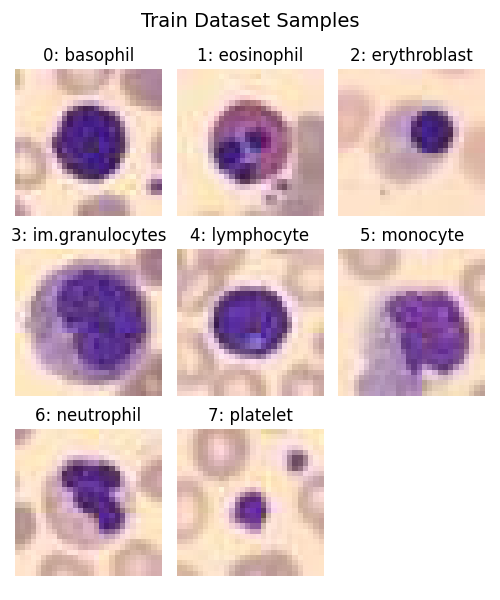
\includegraphics[width=0.95\columnwidth]{Samples_panel.png}
        \caption{Exemplos de imagens por classe.}\label{fig:AmostrasPainel}
    \end{figure}

    Os conjuntos de dados de treino e validação não são uniformemente distribuídos entre as classes (Figura \ref{fig:AmostrasContagem}). Algumas classes tem mais que o dobro de imagens que outras. Prevendo um possível efeito negativo no treinamento, foi proposto utilizar pesos por classe. A proposta foi definir os pesos proporcionais ao inverso do número de classes (Figura \ref{fig:AmostrasPesos}). O impacto do uso de pesos por classe será avaliado para cada classificador.

        \begin{figure}[hbt!]
            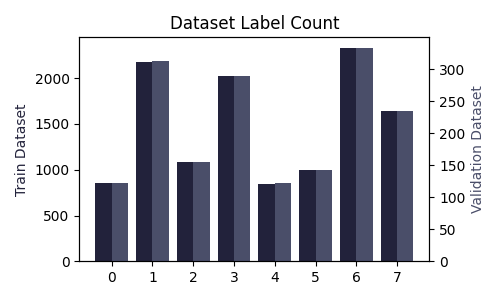
\includegraphics[width=0.95\columnwidth]{Samples_count.png}
            \caption{Número de imagens por classe.}\label{fig:AmostrasContagem}
        \end{figure}

        \begin{figure}[hbt!]
            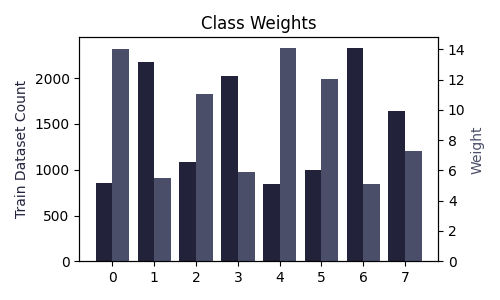
\includegraphics[width=0.95\columnwidth]{Samples_weights.png}
            \caption{Pesos por classe.}\label{fig:AmostrasPesos}
        \end{figure}

    \subsection{Rede MLP}

    O primeiro classificador construído é uma rede neural de uma camada intermediária (\textbf{MLP}). A rede é composta por uma camada de entrada, uma camada intermediária (com função de ativação não-linear) e uma camada de saída (com função de ativação \emph{softmax}).

    Apesar de ser uma rede simples, diferentes hiperparâmetros foram avaliados para tentar encontrar um classificador mais eficiente. A avaliação dos hiperparâmetros foi feita com busca em grade (\emph{GridSearch}). Como o número de possíveis combinações é alto, a busca em grade foi feita por subconjuntos de hiperparâmetros.

    Um conjunto de hiperparâmetros \emph{ótimos} é inicialmente imposto. A partir deste conjunto \emph{ótimo} é feita uma busca em grande com um subconjunto dos hiperparâmetros. Ao final desta busca os valores do conjunto de hiperparâmetros \emph{ótimo} é atualizado com os valores encontrados que maximizam a acurácia do conjunto de validação. O processo é repetido para cada subconjunto de hiperparâmetros.

    A Tabela \ref{tab:ParametrosMLP} mostra os subconjuntos de hiperparâmetros (separados por linhas horizontais). A ordem dos subconjuntos na tabela coincide com a ordem de otimização dos hiperparâmetros.

    A etapa de \emph{data augmentation} testada consistiu de espelhamento (vertical e/ou horizontal) e rotação aleatórios. A descrição da base de dados cita que as imagens estão centradas, de forma que assumiu-se, para este exercício, não ser necessário aplicar a translação aleatória das imagens.

    \begin{table}[h]
        \centering
        \begin{tabular}{l c}
            \toprule
            \textbf{Hiperparâmetro} & \textbf{Opções} \\
            \midrule
            Usar \emph{data augmentation} & \underline{Sim}, Não \\
            Usar pesos por classe & Sim, \underline{Não} \\
            \midrule
            Número de neurônios & 64, \underline{128}, 256, 512, 1024 \\
            \midrule
            Otimizador & \underline{SGD}, RMSprop, Adam \\
            Função de ativação & \underline{relu}, tanh \\
            Tamanho do \emph{batch} & \underline{16}, 32, 64, 128 \\
            \bottomrule
        \end{tabular}
        \caption{Hiperparâmetros da rede MLP (parâmetros ótimos sublinhados).}\label{tab:ParametrosMLP}
    \end{table}

    O ajuste de cada classificador foi feito por até 50 épocas, com parada antecipada (\emph{early stopping}) caso a acurácia\footnote{Como existe certo desbalanceamento entre as classes, a acurácia balanceada possivelmente seria uma métrica melhor, mas esta opção não está facilmente disponível no \emph{TensorFlow}.} dos dados de validação não melhore após 10 épocas (com um mínimo de 20 épocas). O classificador ajustado utiliza os pesos que deram a maior acurácia com os dados de validação durante o processo de ajuste.

    Na busca em grade foi aplicada validação cruzada estratificada em 3 pastas (\emph{StratifiedKFold}) com os dados de treino, com entropia cruzada como função objetivo. A métrica de definição do melhor classificador é a média da acurácia com os dados de validação. Para adequar o custo computacional ao \emph{hardware} disponível, a busca em grade foi limitada a 40\% dos dados de treino e validação.

    A Figura \ref{fig:NeuroniosMLP} mostra o impacto do número de neurônios da camada intermediária na acurácia média com os dados de validação. Existe inicialmente um impacto positivo significativo em aumentar o número de neurônios (\emph{underfitting}). O contínuo incremento leva a uma redução gradativa na qualidade do classificador (\emph{overfitting}).

    A otimização dos hiperparâmetros não foi exaustiva. Outros valores para os hiperparâmetros avaliados, além de outros hiperparâmetros, poderiam ter sido testados, possivelmente encontrando classificadores melhores. Avaliou-se que a otimização feita atende os objetivos do exercício.

     \begin{figure}[hbt!]
         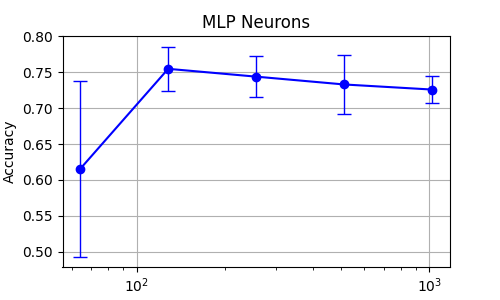
\includegraphics[width=0.95\columnwidth]{MLP_neurons.png}
         \caption{Efeito médio do número de neurônios da camada intermediária na acurácia da rede MLP (barras de erro são iguais a duas vezes o desvio padrão estimado com validação cruzada).}\label{fig:NeuroniosMLP}
     \end{figure}

     Uma nova rede MLP foi treinada com os hiperparâmetros ótimos (Figura \ref{fig:ModeloMLP})\footnote{As figuras maiores foram concentradas no apêndice para facilitar a leitura.}, com um limite 200 épocas. É feita uma parada antecipada se a acurácia dos dados de validação não melhorar após 20 épocas. A Figura \ref{fig:HistoricoMLP} mostra que a rede foi ajustada até a 71\textsuperscript{a} época. Esta rede tem $302\,216$ parâmetros treináveis.

     A acurácia da rede MLP com os dados de teste ficou em $0.7992$. A matriz de confusão (Figura \ref{fig:MatrizConfusaoMLP}) e os resultados por classe (Tabela \ref{tab:ResultadosMLP}) mostram que a distinção de algumas classes foi mais fácil (e.g.: Plaquetas), enquanto que a classificação de outras classes teve desempenho pior (e.g.: Monócitos).

    \begin{figure}[hbt!]
        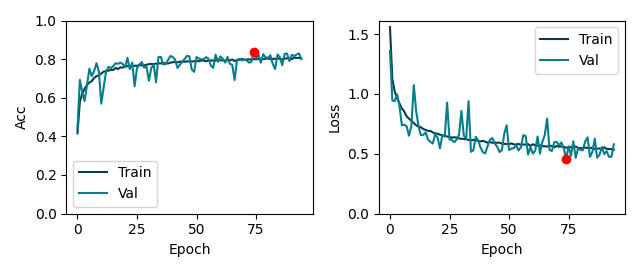
\includegraphics[width=0.95\columnwidth]{MLP_history_cropped.png}
        \caption{Histórico de ajuste da rede MLP.}\label{fig:HistoricoMLP}
    \end{figure}

    \begin{figure}[hbt!]
        \includegraphics[width=0.95\columnwidth]{MLP_cm.png}
        \caption{Matrix de confusão da rede MLP.}\label{fig:MatrizConfusaoMLP}
    \end{figure}

    \begin{table}[h]
        \centering
        \begin{tabular}{l c c}
            \toprule
            \textbf{Classe} & \textbf{Acurácia} \\
            \midrule
            Todas & $0.7992$ \\
            \addlinespace
            Basófilos  & $0.5205$ \\
            Eosinófilos  & $0.9247$ \\
            Eritroblastos  & $0.7878$ \\
            Granulócitos imaturos  & $0.6615$ \\
            Linfócitos  & $0.6749$ \\
            Monócitos  & $0.5599$ \\
            Neutrófilos  & $0.9204$ \\
            Plaquetas  & $0.9915$ \\
            \bottomrule
        \end{tabular}
        \caption{Resultados da rede MLP com os dados de teste.}\label{tab:ResultadosMLP}
    \end{table}

    A Figura \ref{fig:ErrosMLP} exemplifica alguns dos erros de classificação cometidos pelo modelo MLP. Na maioria das classificações errôneas a ordem associada à classe verdadeira é 2 (Figura \ref{fig:HistogramaErrosMLP})\footnote{Cálculo da frequência relativa inclui as classificações corretas (ordem=1), que não é apresentada no gráfico por ter valor muito superior às demais barras.}.

    \begin{figure}[hbt!]
        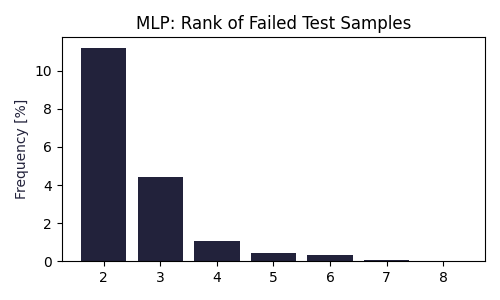
\includegraphics[width=0.95\columnwidth]{MLP_rank.png}
        \caption{Histograma da ordem associada à classe verdadeira para as classificações errôneas com a rede MLP.}\label{fig:HistogramaErrosMLP}
    \end{figure}

    \subsection{Rede Convolucional \emph{Simples}}

    O segundo classificador construído é uma rede neural com uma camada convolucional (\textbf{CNN}). A rede é composta por uma camada de entrada, uma camada convolucional (com função de ativação não-linear), uma camada de \emph{pooling} e uma camada de saída (com função de ativação \emph{softmax}).

    Os critérios (função objetivo, métricas, parada antecipada etc.) e o processo de otimização dos hiperparâmetros e de treinamento da rede CNN foi igual ao aplicado para a rede MLP. A Tabela \ref{tab:ParametrosCNN} mostra os hiperparâmetros avaliados, os agrupamentos feitos e os valores ótimos.

    \begin{table}[h]
        \centering
        \begin{tabular}{l c}
            \toprule
            \textbf{Hiperparâmetro} & \textbf{Opções} \\
            \midrule
            Usar \emph{data augmentation} & \underline{Sim}, Não \\
            Usar pesos por classe & Sim, \underline{Não} \\
            \midrule
            Tamanho dos filtros & \underline{3x3}, 5x5, 7x7 \\
            Número de filtros & 8, 16, 32, 64, \underline{128} \\
            \midrule
            Tamanho do \emph{pooling} & \underline{2}, 3, 4, 5, toda figura\tablefootnote{Equivale a usar as camadas \emph{GlobalMax} e \emph{GlobalAverage} do Keras/Tensorflow.} \\
            Tipo do \emph{pooling} & \underline{máximo}, média\\
            \midrule
            Otimizador & SGD, RMSprop, \underline{Adam} \\
            Função de ativação & \underline{relu}, tanh \\
            Tamanho do \emph{batch} & \underline{16}, 32, 64, 128 \\
            \bottomrule
        \end{tabular}
        \caption{Hiperparâmetros da rede CNN (parâmetros ótimos sublinhados).}\label{tab:ParametrosCNN}
    \end{table}

    A Figura \ref{fig:KernelCNN} mostra o impacto do tamanho dos filtros (\emph{kernel}) e do número de filtros da camada convolucional na acurácia média com os dados de validação. Observa-se que o comportamento não é linear, com o tamanho ótimo do filtro mudando em função do número de filtros.

     \begin{figure}[hbt!]
         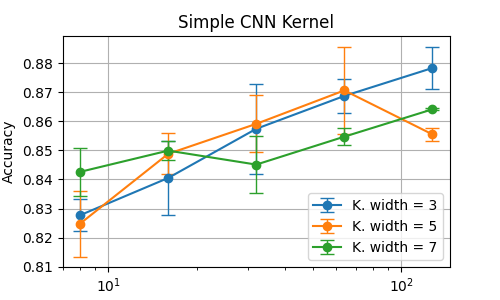
\includegraphics[width=0.95\columnwidth]{CNN_kernel.png}
         \caption{Efeito médio do tamanho dos filtros e do número de filtros da camada convolucional na acurácia da rede CNN.}\label{fig:KernelCNN}
     \end{figure}

     A rede CNN com hiperparâmetros otimizados tem um total de $176\,648$ parâmetros treináveis (Figura \ref{fig:ModeloCNN}). A rede foi ajustada por 70 épocas (Figura \ref{fig:HistoricoMLP}), seguindo a mesma parametrização utilizada para a rede MLP com hiperparâmetros otimizados.

     A acurácia do rede CNN com os dados de teste ficou em $0.9073$. A acurácia teve um significativo incremento comparado com a rede MLP, apesar da rede CNN ter menos parâmetros. A classe Plaquetas teve apenas uma imagem incorretamente classificada (Figura \ref{fig:MatrizConfusaoCNN}). Em comparação com a rede MLP, a rede CNN tem melhor acurácia para todas as classes (Tabela \ref{tab:ResultadosCNN}).

    \begin{figure}[hbt!]
        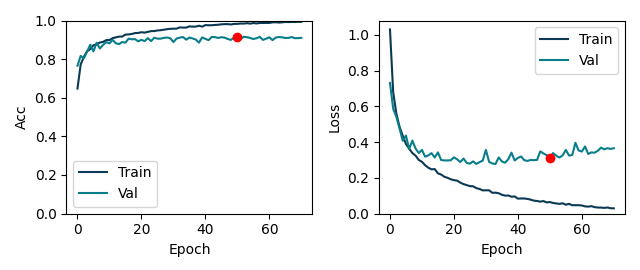
\includegraphics[width=0.95\columnwidth]{CNN_Simple_history_cropped.png}
        \caption{Histórico de ajuste da rede CNN.}\label{fig:HistoricoCNN}
    \end{figure}

    \begin{figure}[hbt!]
        \includegraphics[width=0.95\columnwidth]{CNN_Simple_cm.png}
        \caption{Matrix de confusão da rede CNN.}\label{fig:MatrizConfusaoCNN}
    \end{figure}

    \begin{table}[h]
        \centering
        \begin{tabular}{l c c}
            \toprule
            \textbf{Classe} & \textbf{Acurácia} \\
            \midrule
            Todas & $0.9073$ \\
            \addlinespace
            Basófilos  & $0.7992$ \\
            Eosinófilos  & $0.9792$ \\
            Eritroblastos  & $0.9293$ \\
            Granulócitos imaturos  & $0.8238$ \\
            Linfócitos  & $0.8848$ \\
            Monócitos  & $0.7923$ \\
            Neutrófilos  & $0.9339$ \\
            Plaquetas  & $1.0000$ \\
            \bottomrule
        \end{tabular}
        \caption{Resultados da rede CNN com os dados de teste.}\label{tab:ResultadosCNN}
    \end{table}

    Além de ter um número menor de classificações errôneas, o histograma da ordem associada à classe verdadeira dos dados de teste para a rede CNN (Figura \ref{fig:HistogramaErrosCNN}) se mostra um pouco mais concentrado nos valores menores que o histograma construído com a rede MLP.

    \begin{figure}[hbt!]
        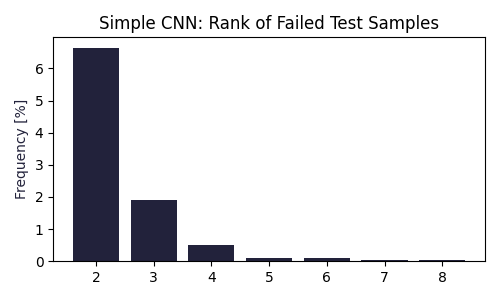
\includegraphics[width=0.95\columnwidth]{CNN_Simple_rank.png}
        \caption{Histograma da ordem associada à classe verdadeira para as classificações errôneas com a rede CNN.}\label{fig:HistogramaErrosCNN}
    \end{figure}

    \subsection{Rede Convolucional \emph{Profunda}}

    A rede convolucional \emph{Profunda} construída se baseou na arquitetura \textbf{\emph{ResNet}} \cite{he2015deep}. A resolução das imagens utilizadas nesta avaliação (28x28) é menor que a das imagens de entrada utilizadas na proposta original das ResNet (224x224). Em função desta diferença no tamanho das imagens, e para evitar uma \emph{explosão} no número de parâmetros, foi construída uma versão simplificada dos blocos propostos para a ResNet-18.

    Dado o alto custo computacional de treinar a rede neural proposta, não foi feita uma otimização dos hiperparâmetros. Os hiperparâmetros foram definidos de forma a limitar o número de parâmetros treináveis. A rede \emph{ResNet} construída consiste de (hiperparâmetros utilizados entre parênteses):

    \begin{enumerate}
        \item Camada convolucional inicial (64 filtros 3x3).
        \item Camada de \emph{max pooling} com janela 3x3 (opção não utilizada).
        \item Blocos residuais (2 blocos):
        \begin{enumerate}
            \item Duplica o número de filtros.
            \item Camada convolucional inicial com \emph{stride} igual a 2 (3x3).
            \item Camadas convolucionais (2 camadas 3x3).
            \item Camada convolucional 1x1 com \emph{stride} igual a 2 aplicada no dado de entrada do bloco residual (\emph{skip connection}).
            \item Soma das saídas das camadas 3x3 com as saídas da camada 1x1.
            \item Aplicada função de ativação (relu).
        \end{enumerate}
        \item Camada de \emph{Global Average Pooling}.
        \item Camada densa (ativação relu).
        \item Camada densa de saída.
    \end{enumerate}

    Todas as camadas convolucionais e de \emph{pooling} utilizam \emph{padding} para buscar manter o tamanho das figuras. Onde não é explícito, foi utilizado \emph{stride} igual a 1. Em todas as camadas a função de ativação é relu, exceto na camada de saída, que utiliza \emph{softmax}. Ao final de cada camada convolucional é feito \emph{batch normalization} antes de aplicar a função de ativação.

    No início de cada bloco residual é duplicado o número de filtros, e o tamanho da figura é reduzido pela metade (\emph{stride} 2 na primeira camada do bloco). Devido à mudança no tamanho da figura, a \emph{skip connection} não utiliza a matriz identidade. É aplicada uma camada convolucional com filtro 1x1 e \emph{stride} 2 para que as saídas tenham mesma dimensão e possam ser somadas.

    Em face dos resultados anteriores, foi utilizado \emph{data augmentation} nesta rede, e não foram utilizados pesos por classe. A rede é apresentada visualmente nas Figuras \ref{fig:ModeloCNNupper} e \ref{fig:ModeloCNNlower}.

    A rede tem $1\,957\,768$ parâmetros treináveis. Foram utilizados os mesmos critérios de ajuste e parada antecipada das redes anteriores. A rede foi ajustada por 102 épocas (Figura \ref{fig:HistoricoResNet}).

    A curva da acurácia com o conjunto de validação tem um comportamento mais \emph{errático} que o observado nos gráficos das demais redes. Este comportamento indica que o critério de parada prematura não é adequado para esta rede mais complexa, e que possivelmente um número maior de épocas levaria a um resultado melhor.

    A acurácia do rede \emph{ResNet} com os dados de teste ficou em $0.9608$. A acurácia teve um novo incremento significativo comparado com as demais redes. Apenas a acurácia da classe Plaquetas não melhorou com relação à rede CNN(Figura \ref{fig:MatrizConfusaoResNet} e Tabela \ref{tab:ResultadosResNet}).

    \begin{figure}[hbt!]
        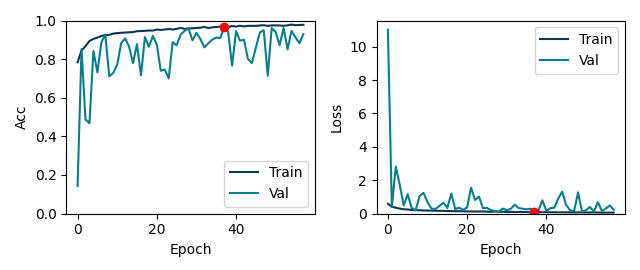
\includegraphics[width=0.95\columnwidth]{ResNet_history_cropped.png}
        \caption{Histórico de ajuste da rede \emph{ResNet}.}\label{fig:HistoricoResNet}
    \end{figure}

    \begin{figure}[hbt!]
        \includegraphics[width=0.95\columnwidth]{ResNet_cm.png}
        \caption{Matrix de confusão da rede \emph{ResNet}.}\label{fig:MatrizConfusaoResNet}
    \end{figure}

    \begin{table}[h]
        \centering
        \begin{tabular}{l c c}
            \toprule
            \textbf{Classe} & \textbf{Acurácia} \\
            \midrule
            Todas & $0.9608$ \\
            \addlinespace
            Basófilos  & $0.9426$ \\
            Eosinófilos  & $0.9968$ \\
            Eritroblastos  & $0.9582$ \\
            Granulócitos imaturos  & $0.9378$ \\
            Linfócitos  & $0.8889$ \\
            Monócitos  & $0.9155$ \\
            Neutrófilos  & $0.9760$ \\
            Plaquetas  & $0.9957$ \\
            \bottomrule
        \end{tabular}
        \caption{Resultados da rede \emph{ResNet} com os dados de teste.}\label{tab:ResultadosResNet}
    \end{table}

    O histograma da ordem associada à classe verdadeira com os dados de teste (Figura \ref{fig:HistogramaErrosResNet}) está mais concentrado nos valores 2 e 3 que os histogramas das demais redes. Este resultado indica que esta rede tem potencial para gerar melhores resultados com uma otimização dos hiperparâmetros e/ou um número maior de épocas no processo de ajuste.

    \begin{figure}[hbt!]
        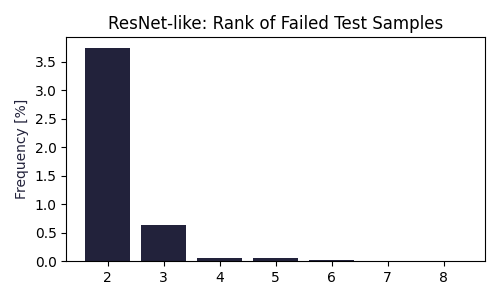
\includegraphics[width=0.95\columnwidth]{ResNet_rank.png}
        \caption{Histograma da ordem associada à classe verdadeira para as classificações errôneas com a rede \emph{ResNet}.}\label{fig:HistogramaErrosResNet}
    \end{figure}

    \section{Conclusão}

    A Tabela \ref{tab:resultados_resumo} resume os resultados principais. Fica claro que, para o problema proposto, é eficiente o uso de camadas convolucionais e de redes residuais profundas. A rede \emph{ResNet} construída não passou por um processo de otimização dos hiperparâmetros ou fez uso de um grande número de camadas, mas a sua acurácia ficou comparável às reportadas para redes mais profundas.

    \begin{table}[h]
        \centering
        \begin{tabular}{l l c}
            \toprule
            \textbf{Rede} & \textbf{Acurácia} \\
            \midrule
            ResNet-18 (28) & $0.958$ \\
            ResNet-18 (224) & $0.963$ \\
            ResNet-50 (28) & $0.956$ \\
            ResNet-50 (224) & $0.950$ \\
            auto-sklearn & $0.878$ \\
            AutoKeras & $0.961$ \\
            Google AutoML Vision & $0.966$ \\
            \midrule
            MLP & $0.799$ \\
            CNN & $0.907$ \\
            \emph{ResNet} & $0.961$ \\
            \bottomrule
        \end{tabular}
        \caption{Resultados reportados na publicação original \cite{medmnistv2} em comparação com as redes construídas nesta atividade.}
        \label{tab:resultados_resumo}
    \end{table}

\appendix

    \section{Redes Neurais Construídas}

        \begin{figure}[H]
            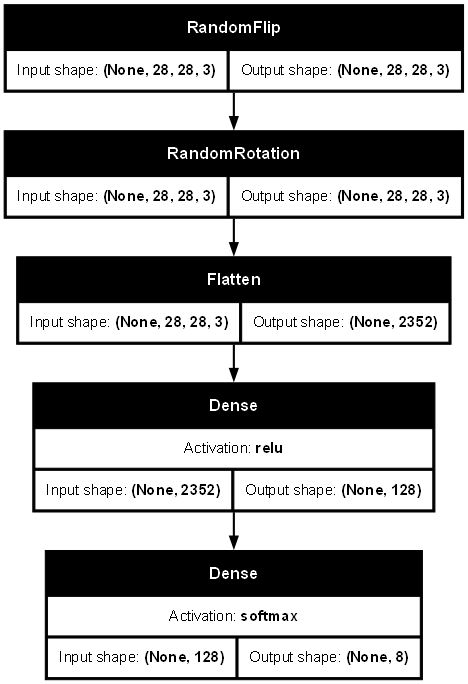
\includegraphics[width=0.95\columnwidth]{MLP_model.png}
            \caption{Rede MLP.}\label{fig:ModeloMLP}
        \end{figure}

        \begin{figure}[H]
            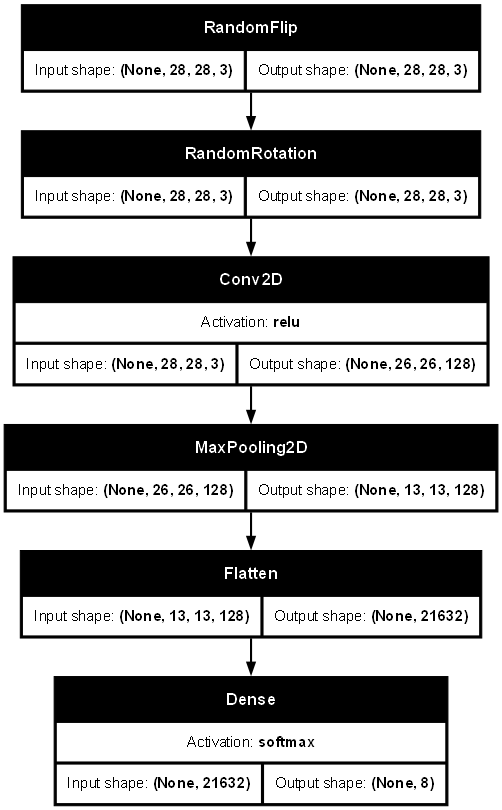
\includegraphics[width=0.95\columnwidth]{CNN_Simple_model.png}
            \caption{Rede CNN.}\label{fig:ModeloCNN}
        \end{figure}

        \begin{figure}[H]
            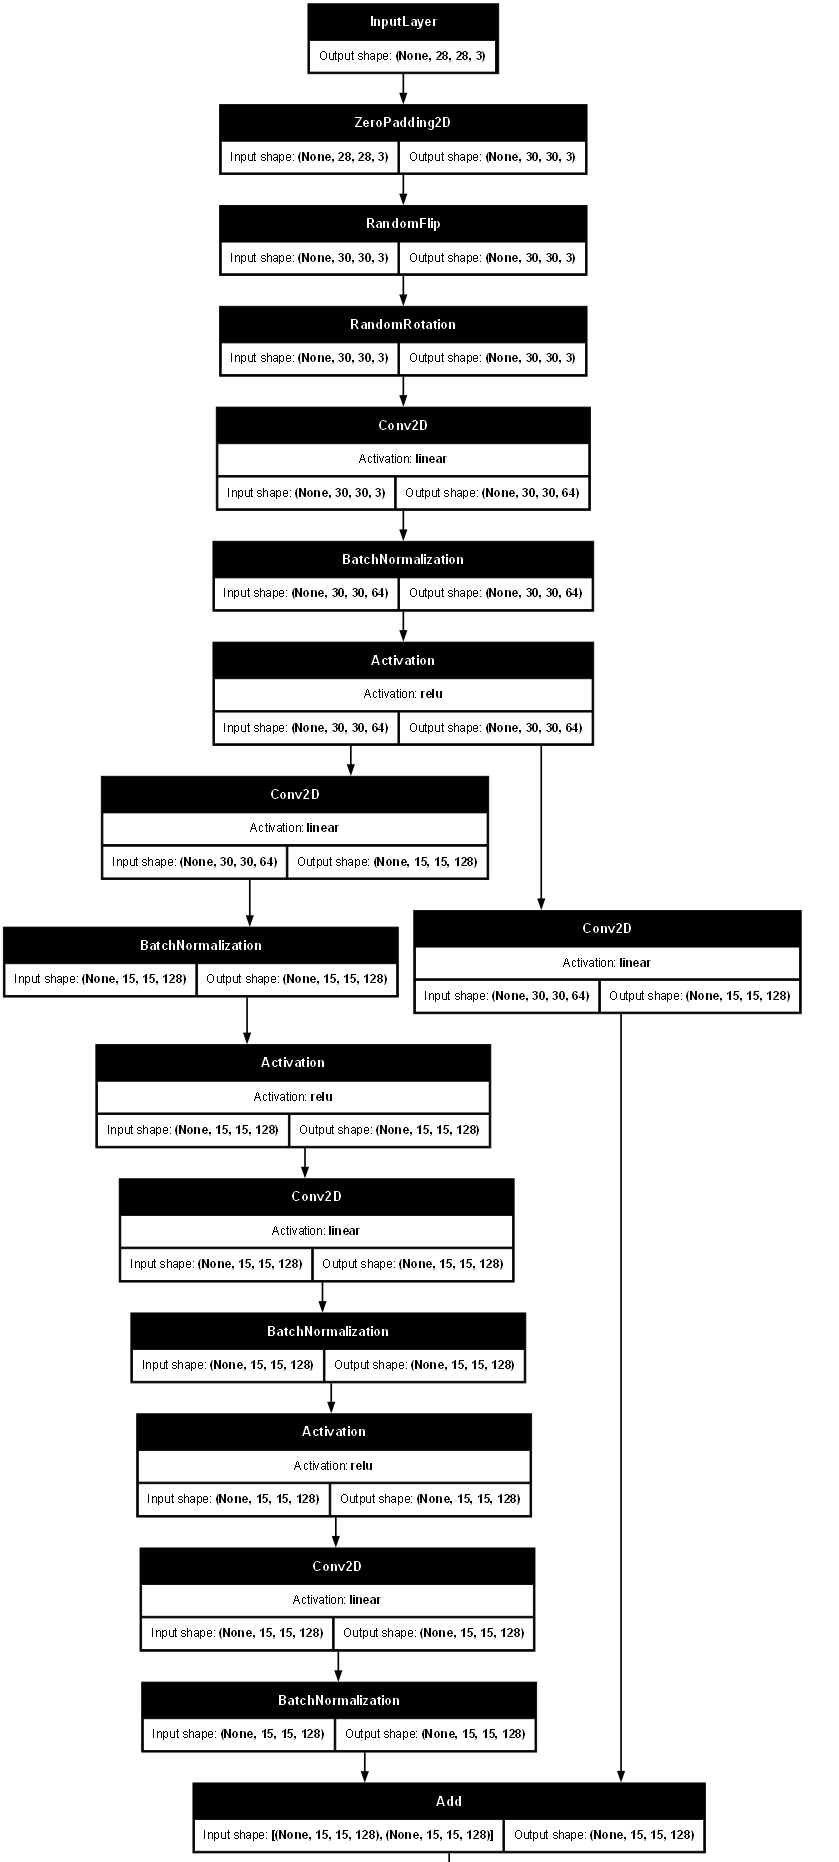
\includegraphics[width=0.95\columnwidth]{ResNet_model_upper.png}
            \caption{Início e primeiro bloco residual da rede \emph{ResNet}.}\label{fig:ModeloCNNupper}
        \end{figure}

        \begin{figure}[H]
            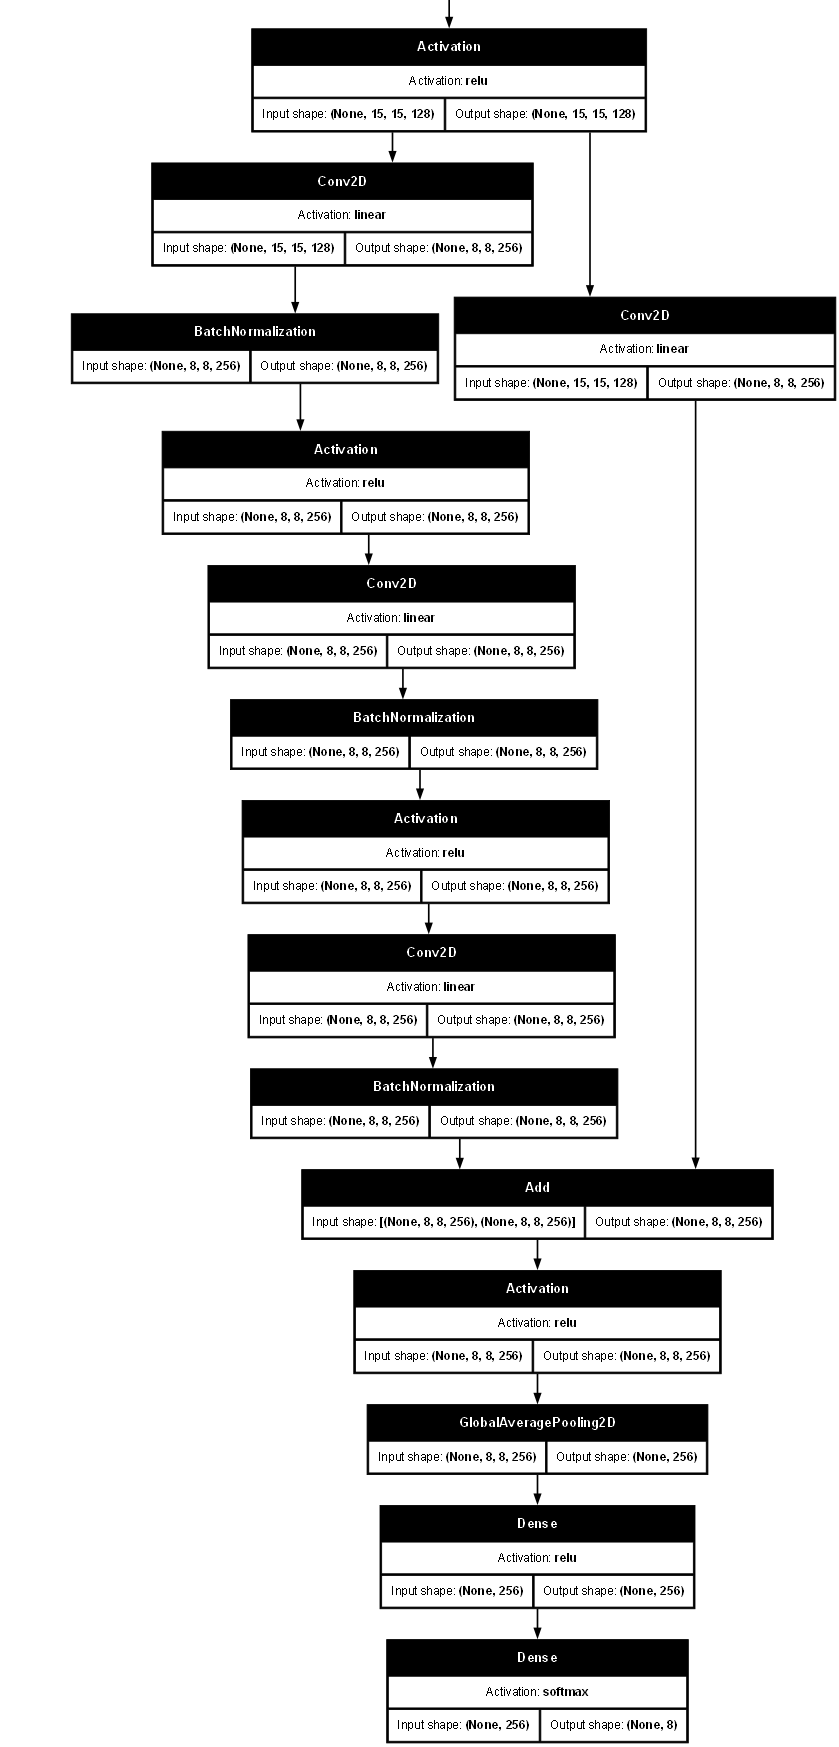
\includegraphics[width=0.95\columnwidth]{ResNet_model_lower.png}
            \caption{Segundo bloco residual e final da rede \emph{ResNet}.}\label{fig:ModeloCNNlower}
        \end{figure}

    \section{Exemplos de Classificações Errôneas}

    À esquerda é apresentada uma figura do conjunto de testes, junto com a sua classificação correta. À direita de cada imagem é apresentada a saída do classificador (probabilidades associadas a cada classe), com a indicação da ordem (\emph{rank}) associada à classe verdadeira.

        \begin{figure}[H]
            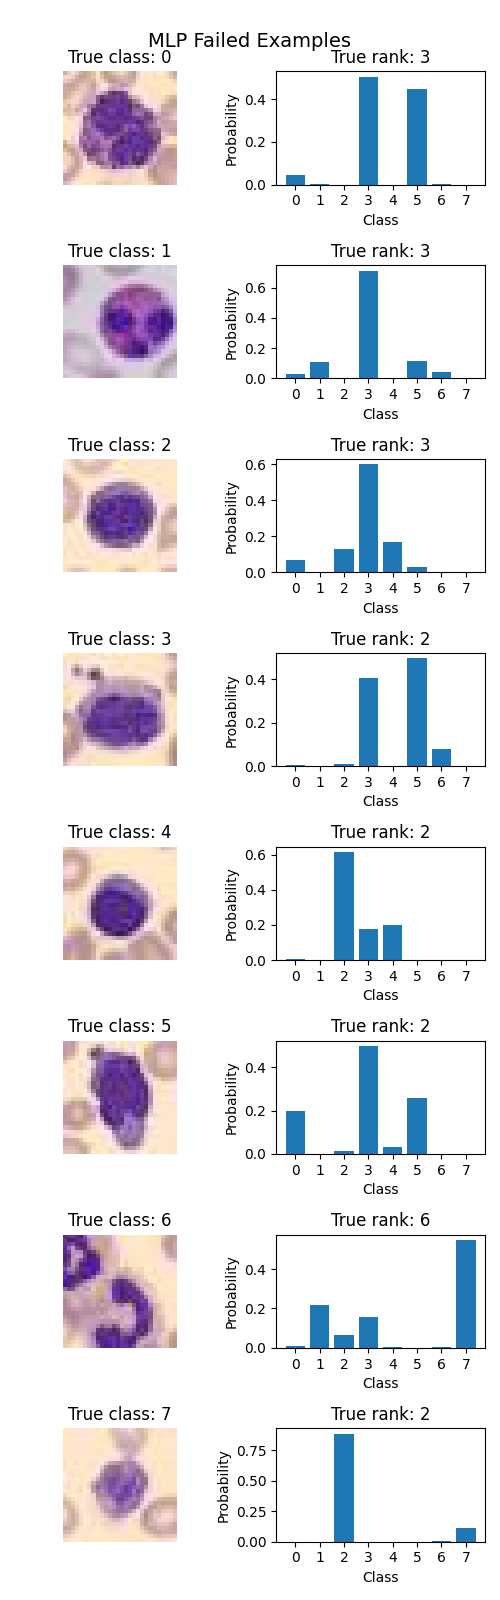
\includegraphics[width=0.8\columnwidth]{MLP_fails.png}
            \caption{Exemplos de classificações errôneas com a rede MLP.}\label{fig:ErrosMLP}
        \end{figure}

        \begin{figure}[H]
            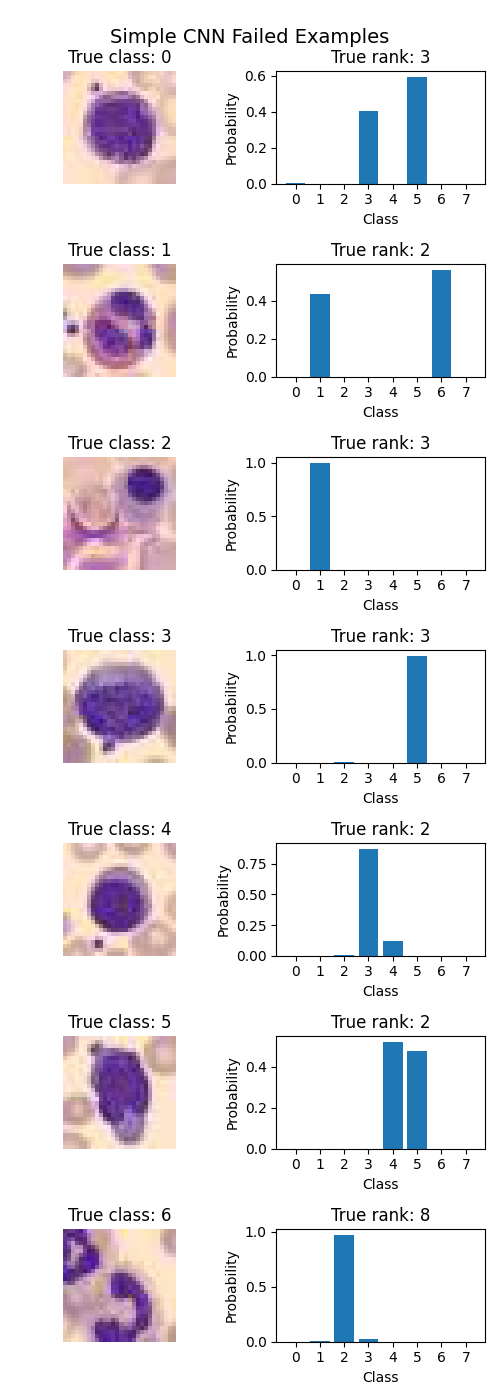
\includegraphics[width=0.8\columnwidth]{CNN_Simple_fails.png}
            \caption{Exemplos de classificações errôneas com a rede CNN.}\label{fig:ErrosCNN}
        \end{figure}

        \begin{figure}[H]
            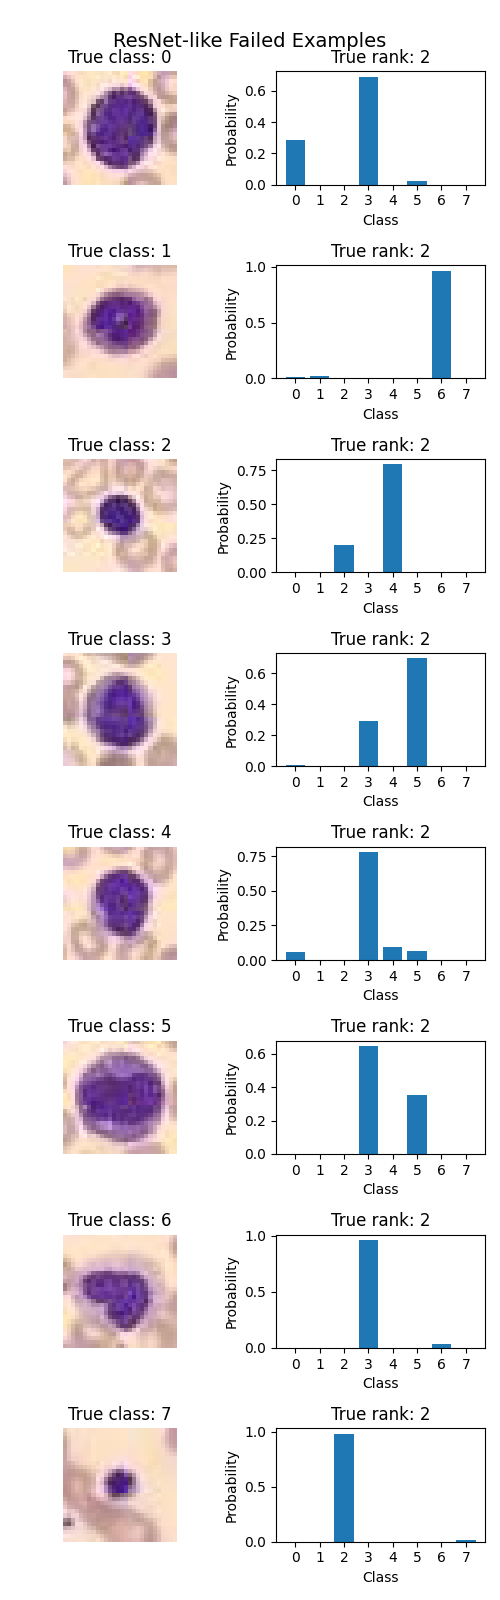
\includegraphics[width=0.8\columnwidth]{ResNet_fails.png}
            \caption{Exemplos de classificações errôneas com a rede \emph{ResNet}.}\label{fig:ErrosResNet}
        \end{figure}

%% \label{}

%% If you have bibdatabase file and want bibtex to generate the
%% bibitems, please use
%%

\bibliographystyle{elsarticle-num}
\bibliography{refs}

%% else use the following coding to input the bibitems directly in the
%% TeX file.

% \begin{thebibliography}{00}

%% \bibitem{label}
%% Text of bibliographic item

% \bibitem{}

% \end{thebibliography}


\end{document}
\endinput
